\section{Pressure}
\label{sec:pressure}

\begin{multicols}{2}


\section*{Concept of Pressure}
%\textbf{Pressure} is the force acting normally per unit surface area. \\
%$\text{Pressure} = \text{Force} \div \text{Area} $


\subsection{What is Pressure?}

\begin{center}
\includegraphics[width=0.49\textwidth]{./img/source/pressure.jpg}
\end{center}

\begin{description*}
%\item[Subtopic:]{}
\item[Materials:]{Pencil, book}
%\item[Setup:]{}
\item[Procedure:]{Ask a student to support a book as shown in figure (a). Then turn the pencil upside down
as shown in figure (b).}
%\item[Hazards:]{}
%\item[Questions:]{}
\item[Observations:]{In case (b) the student will feel pain on the hand supporting the pencil.}
\item[Theory:]{In case (b) the force with which the pencil acts on the hand is the same (equal to the
weight of book plus pencil) as in case (a) but the pressure on the hand has increased very
much since the area on which the pencil touches the hand has decreased so much.}
\item[Applications:]{Large area feet of elephants; wide tyres of tractors; wide chains of caterpillar machines.}
%\item[Notes:]{}
\end{description*}


\subsection{Balloon Pop}

%\begin{center}
%\includegraphics[width=0.4\textwidth]{./img/.png}
%\end{center}

\begin{description*}
%\item[Subtopic:]{}
\item[Materials:]{2 pieces of wood, nails, balloons, water}
\item[Setup:]{Put a single nail through one piece of wood and for the other, put many nails closely spaced. Blow up 2 balloons or fill them with water.}
\item[Procedure:]{Slowly press one balloon against the single nail until it pops. Then repeat for the cluster of nails.}
%\item[Hazards:]{}
%\item[Questions:]{}
\item[Observations:]{The balloon pops easily on the single nail, though it may not pop at all on the cluster of nails.}
\item[Theory:]{Using many nails increases the area over which the force of the nails act, thus decreasing the pressure and requiring a greater force to make the balloon pop.}
%\item[Applications:]{}
\item[Notes:]{You can also hang the balloon from a spring balance as you lower it onto the nails. The difference in weight gives the force needed to pop the balloon.}
\end{description*}

\columnbreak

\subsection{Carrying a Load on the Head}

\begin{center}
\includegraphics[width=0.4\textwidth]{./img/source/load-head.png}
\end{center}

\begin{description*}
%\item[Subtopic:]{}
%\item[Materials:]{}
%\item[Setup:]{}
\item[Procedure:]{Carry a bucket on your head without (a) and with (b) a cloth or khanga.}
%\item[Hazards:]{}
\item[Questions:]{Which is more difficult?}
%\item[Observations:]{}
\item[Theory:]{Using the cloth causes the force of the bucket to be more evenly distributed across a larger area. Hence the force felt at any single point is reduced.}
%\item[Applications:]{}
%\item[Notes:]{}
\end{description*}

\subsection{Potato Poke}

%\begin{center}
%\includegraphics[width=0.4\textwidth]{./img/.png}
%\end{center}

\begin{description*}
%\item[Subtopic:]{}
\item[Materials:]{Straw, potato}
%\item[Setup:]{}
\item[Procedure:]{Try to stab a straw into the potato. Now place your thumb firmly over one end of the straw and try again.}
%\item[Hazards:]{}
%\item[Questions:]{}
\item[Observations:]{The straw bends easily and does not harm the potato the first time. When you cover one end of the straw, it enters the potato easily and may even break through the other side.}
\item[Theory:]{Holding your thumb over the straw traps air inside which increases the pressure in the straw. When it strikes the potato, the increased pressure prevents it from bending and so it is able to poke through the potato.}
%\item[Applications:]{}
%\item[Notes:]{}
\end{description*}

\columnbreak

%==================================================================================================%

\section*{Pressure in Solids}


\subsection[Effect of Surface Area on Pressure]{Effect of Surface Area on \hfill \\ Pressure}

\begin{center}
%\includegraphics[width=0.4\textwidth]{./img/pressure-solid1.png}
%\includegraphics[width=0.4\textwidth]{./img/pressure-solid2.png}
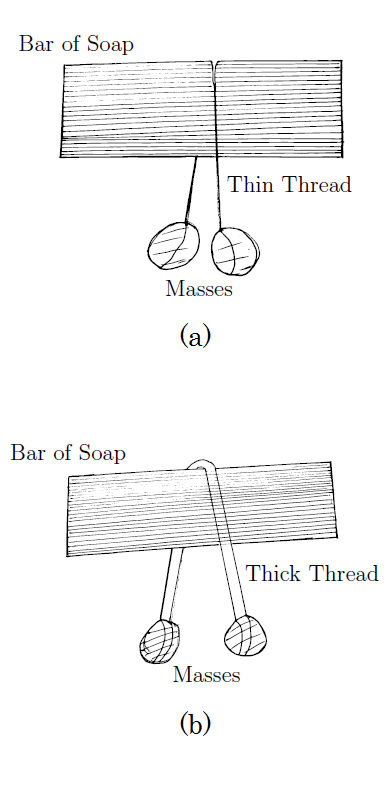
\includegraphics[width=0.4\textwidth]{./img/pressure-solids.png}
\end{center}

\begin{description*}
%\item[Subtopic:]{}
\item[Materials:]{Bar of soap, thin thread, thick string, 4 heavy stones of approximately equal weight}
%\item[Setup:]{}
\item[Procedure:]{Tie a heavy stone to either end of both the thin thread and thick string. Hang each thread across the bar of soap so that the weights hang freely.}
%\item[Hazards:]{}
%\item[Questions:]{}
\item[Observations:]{The thin thread easily cuts through the soap, but the thick string does not.}
\item[Theory:]{The smaller area of the thin thread, acting with the same force, results in an increased pressure which is enough to cut through the soap.}
%\item[Applications:]{}
%\item[Notes:]{}
\end{description*}

\vfill
\columnbreak

%==================================================================================================%

\section*{Pressure in Liquids}


\subsection{Pressure Increases with Depth}

\begin{center}
\includegraphics[width=0.3\textwidth]{./img/source/pressure-depth.png}
\end{center}

\begin{description*}
%\item[Subtopic:]{}
\item[Materials:]{1.5 L bottle, syringe needle or pin/nail, water}
\item[Setup:]{Poke three holes into a bottle. Put one hole near the bottom, one near the middle, and the last hole between them.}
\item[Procedure:]{Fill the bottle with water and place on a table. Observe the trajectories of water coming from the three holes.}
%\item[Hazards:]{}
\item[Questions:]{Which stream goes the farthest distance horizontally? Which hole has the highest pressure?}
\item[Observations:]{The water flowing from the lower holes travels farther.}
\item[Theory:]{The added weight of the water above the lower holes increases the pressure there, resulting in an increased horizontal velocity. It is shown that pressure increases with depth ($P = \rho g h$).}
\item[Applications:]{The wall of a dam is made much thicker at the bottom than at the top. This is to reinforce against the increased water pressure at greater depths.}
%\item[Notes:]{}
\end{description*}

\subsection{Pressure Acts in All Directions}

\begin{center}
\includegraphics[width=0.4\textwidth]{./img/source/pressure-direction.png}
\end{center}

\begin{description*}
%\item[Subtopic:]{}
\item[Materials:]{Water bottle/balloon/plastic bag, pin/needle, water}
%\item[Setup:]{}
\item[Procedure:]{Fill a bottle, balloon or plastic bag with water. Poke several small holes around the surface.}
%\item[Hazards:]{}
%\item[Questions:]{}
\item[Observations:]{Water is expelled equally through all of the holes.}
\item[Theory:]{Pressure in a liquid acts equally in all directions.}
%\item[Applications:]{}
%\item[Notes:]{}
\end{description*}

\subsection{Straw Fountain}

\begin{center}
\includegraphics[width=0.25\textwidth]{./img/vso/straw-fountain.jpg}
\end{center}

\begin{description*}
%\item[Subtopic:]{}
\item[Materials:]{500 mL water bottle with cap, water, straw, glue, hot nail/pin}
\item[Setup:]{Poke a hole the size of the straw in the bottle cap using a heated nail or pin. Stick the straw through the hole and screw on the cap so that the straw reaches near the bottom. Glue around the straw so that it is air tight.}
\item[Procedure:]{Fill the bottle about half way with water and close the cap with the straw inside. Have a student blow as hard as they can through the straw into the water and then stop.}
%\item[Hazards:]{}
%\item[Questions:]{}
\item[Observations:]{When the student stops blowing, they get sprayed in the face by water.}
\item[Theory:]{Blowing into the bottle greatly increases the pressure inside. When you stop blowing, the pressure equalizes by forcing water back out through the straw.}
%\item[Applications:]{}
%\item[Notes:]{}
\end{description*}

\subsection{Hydraulic Press}

\begin{center}
\includegraphics[width=0.3\textwidth]{./img/source/hydraulic-press.png}
\end{center}

\columnbreak

\begin{description*}
%\item[Subtopic:]{}
\item[Materials:]{2 syringes of different size (5 mL and 20 mL), \nameref{sec:delivery-tube}, water}
\item[Setup:]{Fill the larger syringe with water and attach one end of the rubber tubing to its end. Attach the other end of the tubing to the smaller syringe (with its plunger inserted all the way).}
\item[Procedure:]{Pushing the plunger of the larger syringe will cause the plunger of the smaller syringe to go out, and vice-versa.}
%\item[Hazards:]{}
%\item[Questions:]{}
\item[Observations:]{It is easier to push the plunger of the small syringe than that of the larger syringe.}
\item[Theory:]{Pascal's principle states that pressure is distributed equally throughout a liquid. Thus, the pressure at one plunger must be equal to the pressure at the other plunger. Setting the two ratios equal, we can see that a small force over a small area can overcome a large force over a large area.}
\item[Applications:]{Industrial machinery, hydraulic breaks}
%\item[Notes:]{}
\end{description*}

\subsection{The Manometer}

\begin{center}
\includegraphics[width=0.48\textwidth]{./img/source/manometer.png}
\end{center}

\begin{description*}
%\item[Subtopic:]{}
\item[Materials:]{\nameref{sec:delivery-tube}, ruler, cardboard, string, water, food colour, water bottle}
\item[Setup:]{Create the manometer as shown by attaching thin tubing in a U-shape to a cardboard stand and filling with a small amount of coloured water. Make sure there is sufficient length of tubing left over on either side.}
\item[Procedure:]{Insert each arm of the manometer to a different depth in a bottle of water.}
%\item[Hazards:]{}
%\item[Questions:]{}
\item[Observations:]{When both arms are at equal pressure, the water levels are equal. When one side experiences a higher pressure, there is a noticeable difference in the height $h$ of coloured water on the opposite side.}
\item[Theory:]{A manometer is used to measure fluid pressure. When the pressure is higher on one side, it is shown by a difference in height on the manometer which can be measured. The greater the pressure difference, the higher the value of $h$.}
%\item[Applications:]{}
%\item[Notes:]{}
\end{description*}

%==================================================================================================%

\section*{Atmospheric Pressure}
\label{sec:atm-pressure}


\subsection{Overturned Glass}

\begin{center}
\includegraphics[width=0.4\textwidth]{./img/source/overturned-glass.png}
\end{center}

\begin{description*}
%\item[Subtopic:]{}
\item[Materials:]{Cup/glass, card, water}
%\item[Setup:]{}
\item[Procedure:]{Fill a cup to the rim with water. Push a smooth card from the side to cover the glass so that no air bubbles are included. Turn the glass upside down.}
%\item[Hazards:]{}
\item[Questions:]{Why can there be no air bubbles inside the glass?}
\item[Observations:]{The card remains attached to the glass and the water does not fall out.}
\item[Theory:]{The card is held in place by atmospheric pressure pushing upwards, which is larger than the weight of the water pushing downwards, so the card does not fall.}
%\item[Applications:]{}
%\item[Notes:]{}
\end{description*}

\subsection{Holey Bottle}

%\begin{center}
%\includegraphics[width=0.4\textwidth]{./img/.png}
%\end{center}

\begin{description*}
%\item[Subtopic:]{}
\item[Materials:]{Water bottle, pin, water}
%\item[Setup:]{}
\item[Procedure:]{Poke 4 or 5 small holes in the bottom of the bottle. Fill it half way with water, allowing it to spill out the holes in the bottom. Then cap the bottle and observe what happens.}
%\item[Hazards:]{}
%\item[Questions:]{}
\item[Observations:]{When the bottle is capped, the water stops flowing through the holes.}
\item[Theory:]{When the bottle is open, gravity is strong enough to pull the water through the bottom holes. When closed, however, the low pressure inside the bottle and the high atmospheric pressure outside creates an upward force that is able to overcome gravity and prevent water from flowing.}
%\item[Applications:]{}
%\item[Notes:]{}
\end{description*}

\subsection{Bottle Crush}

\begin{center}
\includegraphics[width=0.45\textwidth]{./img/source/bottle-crush.png}
\end{center}

\begin{description*}
%\item[Subtopic:]{}
\item[Materials:]{Plastic water bottle, boiling water, cold water}
%\item[Setup:]{}
\item[Procedure:]{Pour some boiling water into the bottle and cap it immediately. Shake it to make sure all the air inside is heated. Then pour cold water on the bottle.}
%\item[Hazards:]{}
%\item[Questions:]{}
\item[Observations:]{Upon pouring the cold water, the bottle crushes.}
\item[Theory:]{When the hot air inside the water bottle is cooled off, its volume decreases, leaving a partial vacuum inside the bottle. The greater atmospheric pressure outside crushes the bottle inwards.}
%\item[Applications:]{}
%\item[Notes:]{This is an application of Charles' Law. For more, see \nameref{}.}
\end{description*}

\subsection{Automatic Flushing Tank}
\label{sub:auto-tank}

\begin{center}
\includegraphics[width=0.25\textwidth]{./img/auto-flushing-tank.png}
\end{center}

\begin{description*}
%\item[Subtopic:]{}
\item[Materials:]{Empty water bottle, straw, water, bucket, super glue}
\item[Setup:]{Cut the top off of a water bottle and make a hole at the bottom for a straw to fit through. Bend the straw inside the bottle as shown and seal with super glue.}
\item[Procedure:]{Fill the bottle up to and above the bend in the straw and observe what happens.}
%\item[Hazards:]{}
%\item[Questions:]{}
\item[Observations:]{The water will flow into the bucket through the bent straw.}
\item[Theory:]{The combined pressure of the water and the atmosphere pushing down on the water is greater then the air pushing up on the straw. The tank does not require a handle to trigger the flush. Once the water flows into the tank up to the level of the siphon, the tank will flush automatically. }
%\item[Applications:]{}
%\item[Notes:]{}
\end{description*}

\columnbreak

\subsection{The Barometer}

\begin{center}
\includegraphics[width=0.3\textwidth]{./img/source/barometer.png}
\end{center}

\begin{description*}
%\item[Subtopic:]{}
\item[Materials:]{Bottle, plastic bag, string/rubber band, straw, glue, cardboard, pen}
%\item[Setup:]{}
\item[Procedure:]{Close a bottle air-tight using a piece of plastic bag and string/rubber band. Glue the straw onto the middle of the plastic and point it to a vertical scale written on paper or cardboard.}
%\item[Hazards:]{}
%\item[Questions:]{}
%\item[Observations:]{}
\item[Theory:]{When the air pressure increases, it pushes downward on the plastic and the straw dips down. When the air pressure decreases, the relatively high pressure inside the bottle pushes the plastic up, raising the straw.}
%\item[Applications:]{}
%\item[Notes:]{}
\end{description*}

\subsection{Madgeburg Hemisphere}

%\begin{center}
%\includegraphics[width=0.4\textwidth]{./img/.png}
%\end{center}

\begin{description*}
%\item[Subtopic:]{}
\item[Materials:]{2 equal size cooking pots, oil, matches, small pieces of paper}
\item[Setup:]{Spread oil or grease around the edge of one of the cooking pots.}
\item[Procedure:]{Place small papers in the un-greased pot and light them on fire. Allow them to burn about half way and then cover with the greased pot so that no air can escape. Allow the pots to cool and try to separate them.}
%\item[Hazards:]{}
%\item[Questions:]{}
\item[Observations:]{After the pots have cooled it is very difficult to separate them.}
\item[Theory:]{When you burn the paper, the air in the pot expands and escapes. When you cover the pots, no more air can enter and the air inside cools, reducing the pressure inside the pots while the pressure outside the pots remains the same. The atmospheric pressure therefore presses the pots together so as to equalize the pressure on either side. }
%\item[Applications:]{}
%\item[Notes:]{}
\end{description*}

\columnbreak

%==================================================================================================%

\section*{Applications of Atmospheric Pressure}


\subsection{The Siphon}

\begin{center}
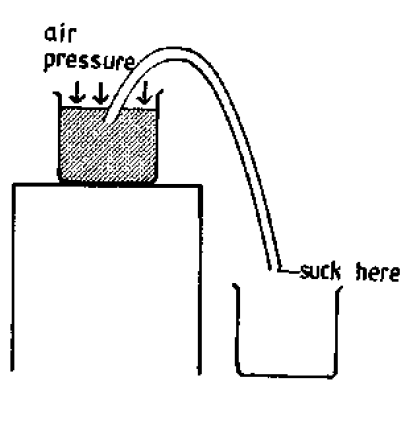
\includegraphics[width=0.4\textwidth]{./img/source/siphon.png}
\end{center}

\begin{description*}
%\item[Subtopic:]{}
\item[Materials:]{2 containers/bottles, \nameref{sec:delivery-tube}, (1 m), water}
%\item[Setup:]{}
\item[Procedure:]{Place one bottle full of water on a table and the other below. Place one end of the tubing into the water and suck on the other end until water starts coming out. Place this end of the tube into the empty bottle and observe what happens.}
\item[Hazards:]{Clean off the tube thoroughly between uses.}
%\item[Questions:]{}
\item[Observations:]{The water continues to flow to the empty bottle despite an initial uphill climb.}
\item[Theory:]{Sucking on the tube creates a low pressure on that end. The higher atmospheric pressure on the water end causes the water to flow from high pressure to low pressure, overcoming gravity.}
\item[Applications:]{Toilets, drainage systems, \nameref{sub:auto-tank}}
\item[Notes:]{Alternatively, submerge the entire tube initially, then pinch on end and remove from the water. Upon releasing the pinched end outside of the water, the water will flow.}
\end{description*}

%\subsection{Reverse Air Pump} %?%
%
%\begin{center}
%\includegraphics[width=0.4\textwidth]{./img/.png}
%\end{center}
%
%\begin{description*}
%%\item[Subtopic:]{}
%\item[Materials:]{}
%\item[Setup:]{}
%\item[Procedure:]{}
%\item[Hazards:]{}
%\item[Questions:]{}
%\item[Observations:]{}
%\item[Theory:]{}
%\item[Applications:]{}
%\item[Notes:]{}
%\end{description*}

%\subsection{Reverse Air Pump}
%\begin{itemize}
%\item{Preparation Time: varies, about 1 hour}
%\item{Materials: Bicycle pump (the tall, metal kind), short piece of rubber tubing fitted to pump valves, utility knife, tightening sleeves, extra valve}
%\item{Procedure: There are two parts of the pump that control the direction of airflow: the first is a diaphragm inside the pump and the second is a ball valve at the base of the pump in the hose.
%\begin{enumerate}
%\item{You need to open the pump and pull out the ‘dipstick’ with the diaphragm attached. At the bottom, there should be a diaphragm with holes around the top, a metal disc the same diameter as the diaphragm, and a few nuts and washers to keep it all together. In its normal configuration, the diaphragm is pulled down by friction away from the disc when the pump handle is pulled up, allowing air to enter the pump freely. When the pump handle is pushed in, the diaphragm is forced against the disc, restricting any back airflow, and forcing all the air forward through the hose. Switch the position and direction of the diaphragm and disc so that it has the opposite effect when the pump handle is pulled in or out.}
%\item{Next, you need to cut open the hose at the base of the pump and find the valve with the small bead inside. Normally, when air is forced forward through the valve, the bead does not restrict any airflow. When air tries to go back through the pump, the bead blocks the valve and stops any airflow. Switch the direction of the valve.}
%\item{From here, you need to reattach the hose to the pump. You may need to get another nozzle to attach to the pump, attaching the hose with reversed valve with the extra bit of rubber tubing. It depends on your pump, but if you have made it this far, you will find a way to make it work. Tightening sleeves will come in handy here to make sure no air is lost after all this cutting and jury-rigging.}
%\end{enumerate}
%} % Procedure
%\item{Applications: This suction pump is great for showing the gas laws and boiling points: suck the air out of a jar of water and watch the water boil, you could also kill stuff in the jar this way, but that is just morbid, and possibly cool, or that sound travels through a medium.}
%\end{itemize}


\end{multicols}

\pagebreak